\documentclass[a4paper,12pt]{article}
\usepackage{outline}
\usepackage{pmgraph}
\usepackage[normalem]{ulem}
\usepackage{comment} % enables the use of multi-line comments (\ifx \fi)
\usepackage{lipsum} %This package just generates Lorem Ipsum filler text.
\usepackage{fullpage} % changes the margin
\usepackage{listings}
\usepackage{color}
\usepackage{mdframed}
\usepackage{listings}
\usepackage{graphicx}
\graphicspath{ {../} }
\renewcommand{\lstlistingname}{Code Block}% Listing -> Algorithm
\renewcommand{\lstlistlistingname}{List of \lstlistingname s}% List of Listings -> List of Algorithms
\title{\textbf{Lab 06: Introduction to Logic Simulation and Verilog}}
\author{Joseph Martinsen \\ ECEN 248-510 \\ TA: Michael Bass}
\date{\today}

\linespread{1.5}
%--------------------Indention
\setlength{\parindent}{15pt}
\lstset{frame=shadowbox, rulesepcolor=\color{white}}
\mdfsetup{frametitlealignment=\center}
\lstset{
  numbers=left,
  stepnumber=1,
  firstnumber=1,
  numberfirstline=true
}

\begin{document}
\section*{Objective}
\hspace{15pt}The purpose of this lab was to move from a total bread board circuit and towards learning and appreciating how modern digital design is implemented. This lab will expose students to Verilog. The student will construct in Verilog some of the circuits from the previous labs including a 1-bit wide, 2:1 multiplexer, a full adder, a ripple carry adder, a 4-bit wide, 2:1 multiplexer and finally a 4-bit Arithmetic Logic Unit. Some Linux knowledge will be thrown in for good measure.

\section*{Design}
\textbf{Experiment 1}
\vspace{5pt}

For \textbf{Experiment 1}, the ISE Project Navigator was set up and a simple 1-bit 2:1 multiplexer module was created \textit{(see Code Block 1)}. This module was a basic first introduction into the world of Verilog. Once written, it was then ran with a supplied test bench file.

\lstinputlisting[language=Verilog,caption=1-bit 2:1 MUX]{../two_one_mux.v}
\vspace{5pt}

\hspace{-15pt}\textbf{Experiment 2}
\vspace{5pt}

\textbf{Experiment 2} consisted of creating three modules in order to build a simple 4-bit ALU later on in \textbf{Experiment 3}. The first component was building upon the 1-bit 2:1 MUX from earlier and creating a 4 bit 2:1 MUX by combing two  1-bit 2:1 MUXs \textit{(see Code Block 2)}. This module was then tested against the supplied full a test bench.

\lstinputlisting[language=Verilog,,caption=4-bit 2:1 MUX]{../four_bit_mux.v}

Next, a full adder module was created. This module functioned with the same logic as previously built full adders. This module \textit{(Code Block 3)} included the first uses of assign for the student. This module was then tested against the supplied full adder test bench.

\lstinputlisting[language=Verilog,,caption=Full Adder]{../full_adder.v}

Finally, an Addition/Subtraction unit was designed much like the !addition/subtraction from the full adder in Lab 05. This unit included the previously created full adder in order to make a ripple carry adder. This module \textit{Code Block 4} was then tested against the supplied Add-Sub test bench.

\lstinputlisting[language=Verilog,,caption=Add Sub Module]{../add_sub.v}
\vspace{5pt}

\hspace{-15pt}\textbf{Experiment 3}

In the final experiment, all the parts from \textbf{Experiment 2} were incorporated in order to create a 4-bit ALU. This module specifically utilizied the 4-bit MUX module as well as the add sum module. This final 4-bit ALU module \textit{(Code Block 5)}, was then tested against the 4-bit ALU test bench.

\lstinputlisting[language=Verilog,,caption=4-Bit ALU ]{../four_bit_alu.v}

\section*{Results}

\hspace{15pt}The following inclued an image of the test results and another image for the waveforms captured during simmulation.

\hspace{-15pt}\textbf{Experiment 1}

\begin{figure}[h]
  \begin{center}
    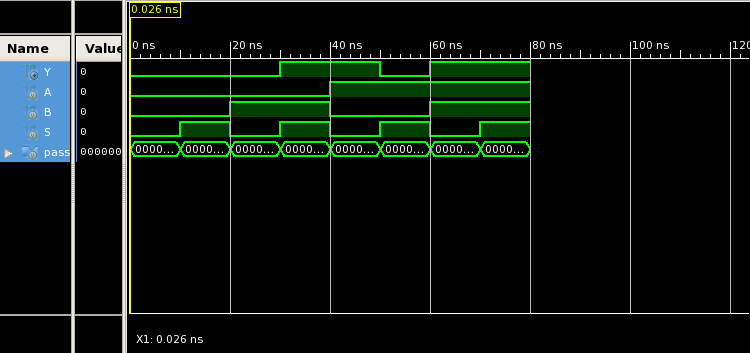
\includegraphics[scale=1]{2_1MuxPlot.png}
    \caption{\textit{2-Bit 2:1 MUX Plots}}
  \end{center}
\end{figure}

\begin{figure}[h]
  \begin{center}
    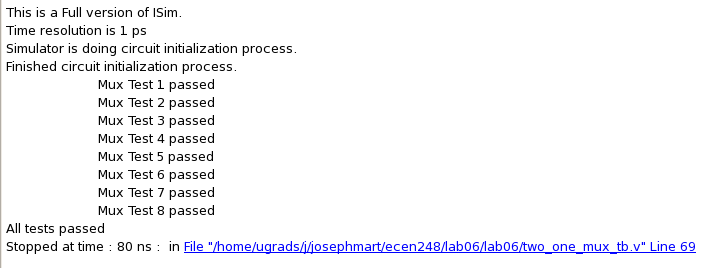
\includegraphics[scale=1]{2_1MuxTests.png}
    \caption{\textit{2-Bit 2:1 MUX Tests}}
  \end{center}
\end{figure}

\newpage

\hspace{-15pt}\textbf{Experiment 2}

\begin{figure}[h]
  \begin{center}
    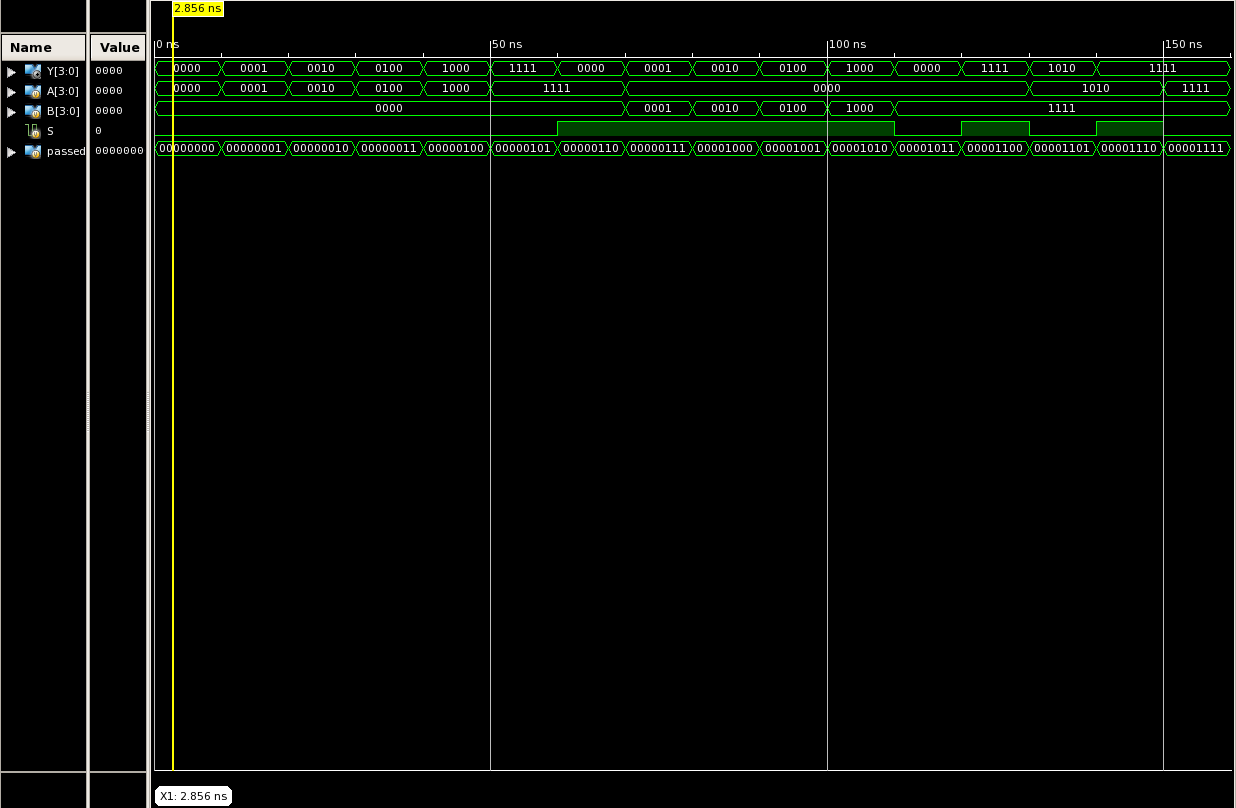
\includegraphics[scale=0.5]{4_1MuxPlot.png}
    \caption{\textit{4-Bit 2:1 MUX Plot}}
  \end{center}
\end{figure}

\begin{figure}[h]
  \begin{center}
    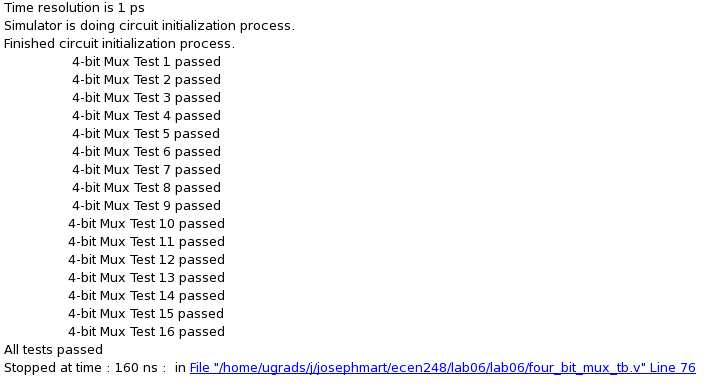
\includegraphics[scale=0.65]{4_1MuxTests.png}
    \caption{\textit{4-Bit 2:1 MUX Tests}}
  \end{center}
\end{figure}

\newpage

\begin{figure}[h]
  \begin{center}
    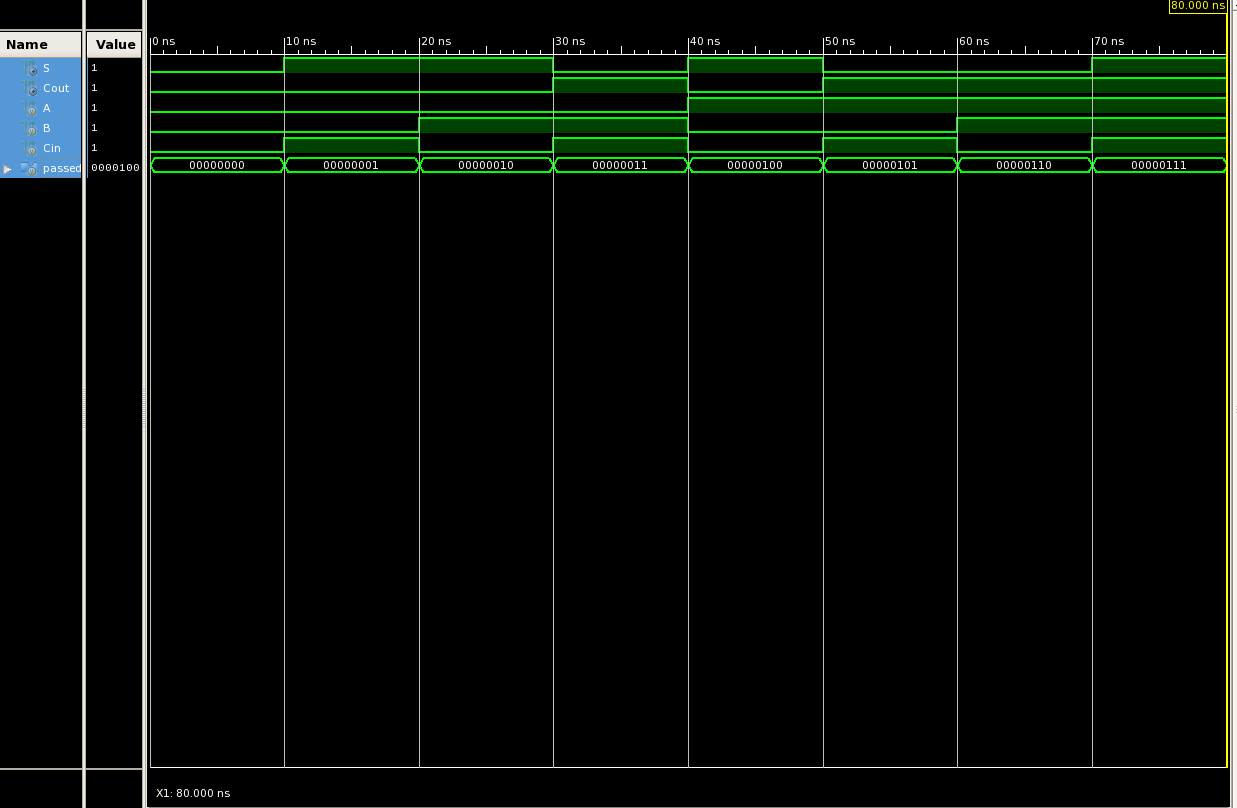
\includegraphics[scale=0.6]{FullAdderPlots.png}
    \caption{\textit{Full Adder Tests}}
  \end{center}
\end{figure}

\begin{figure}[h]
  \begin{center}
    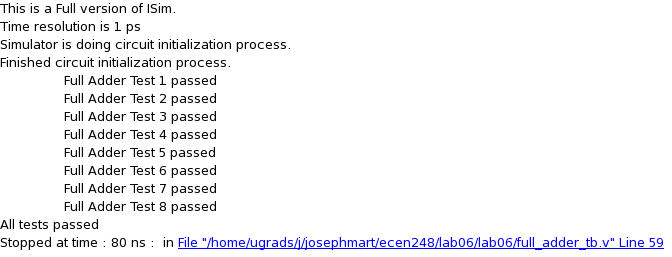
\includegraphics[scale=0.65]{FullAdderTests.png}
    \caption{\textit{Full Adder Tests}}
  \end{center}
\end{figure}

\newpage

\begin{figure}[h]
  \begin{center}
    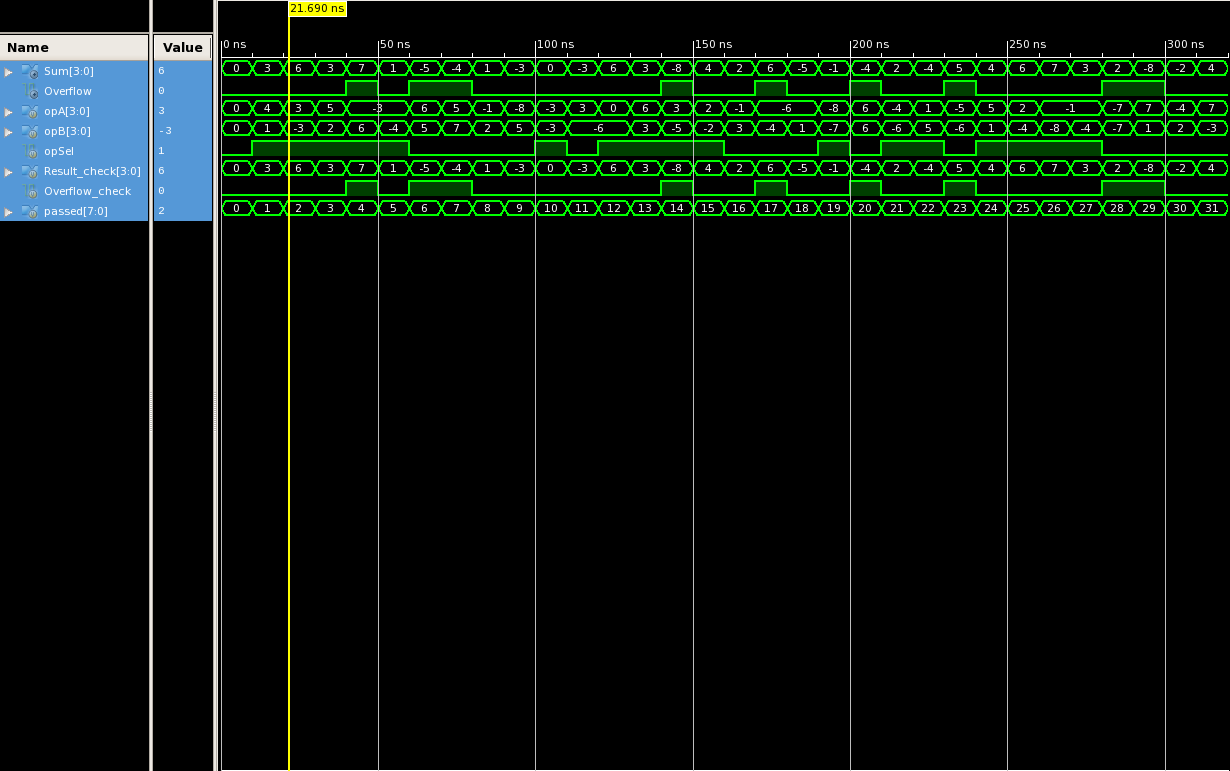
\includegraphics[scale=0.4]{Add_SubPlot.png}
    \caption{\textit{Add/Sub Tests}}
  \end{center}
\end{figure}

\begin{figure}[h]
  \begin{center}
    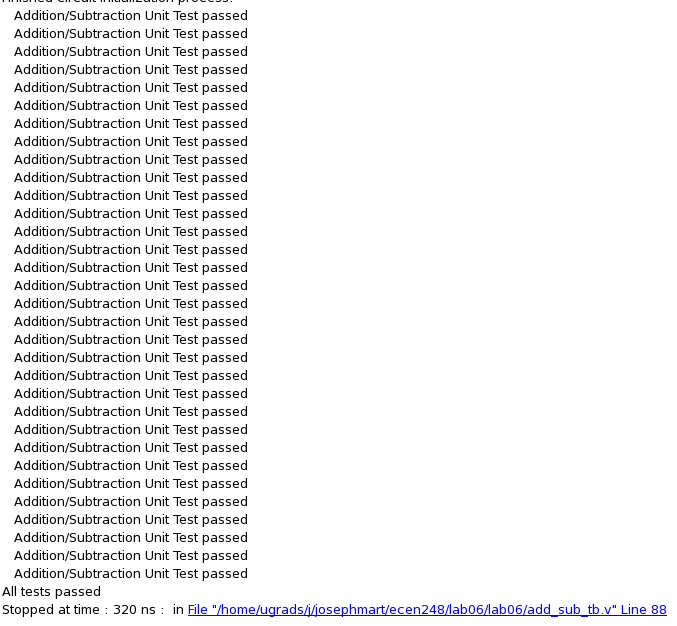
\includegraphics[scale=0.5]{Add_SubTests.png}
    \caption{\textit{Add/Sub Tests}}
  \end{center}
\end{figure}
\newpage
\hspace{-15pt}\textbf{Experiment 3}
\begin{figure}[h]
  \begin{center}
    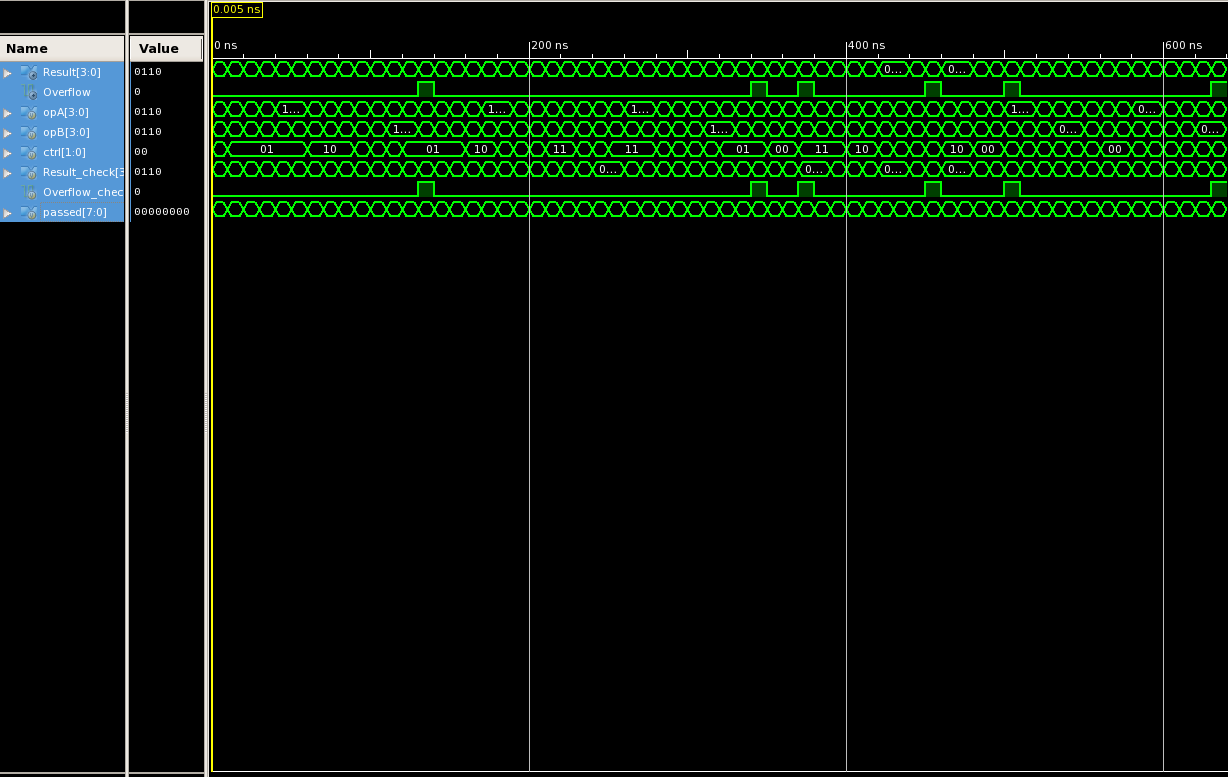
\includegraphics[scale=0.4]{ALUPlots.png}
    \caption{\textit{ALU Plot}}
  \end{center}
\end{figure}

\begin{figure}[h]
  \begin{center}
    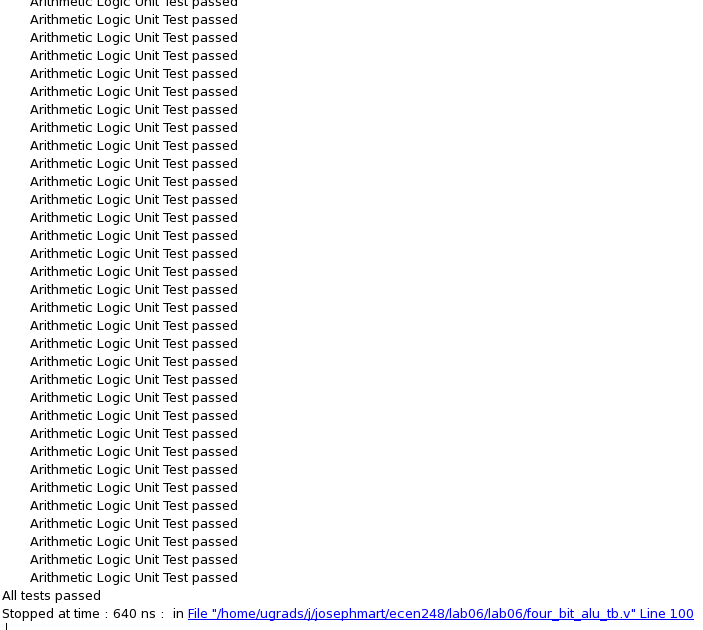
\includegraphics[scale=0.55]{ALUTests.png}
    \caption{\textit{ALU Test}}
  \end{center}
\end{figure}

\section*{Conclutions}

\hspace{15pt}In this lab, Verilog was used in lab for the very first time. This lab was very different from the previous labs because no breadboards or wires were used. Also, I was able to finish this lab. This lab was similar to previous labs because the circuitry and logic exactly the same. The labs were just converted and implemented in a Verilog format.

\section*{Questions}

\begin{enumerate}
  \item \textbf{Include the source code with comments for all modules you simulated. You do not have to include test bench code. Code without comments will not be accepted!}
  \vspace{10pt}

  \textit{In the report}

  \item \textbf{Include screenshots of all waveforms captured during simulation in addition to the test bench console output for each test bench simulation.}
  %\vspace{1pt}

  \textit{In the report}

  \item \textbf{Examine the 1-bit, 2:1 MUX test bench code. Attempt to understand what is going on in the code. The test bench is written using behavior Verilog, which will read much like a programming language. Explain briefly what it is the test bench is doing.}
  \vspace{10pt}

  The test bench code begins by first creating two tasks. The task looks similiar to a function. The task takes in the output of the student created MUX and compares it to the
  correct value and lets the user know if they passed or fail a particular test. If the user passed all the tests, let the
  user know. Next, the wires and MUX is initialized. Finally the
  output values are compared to actual values through the
  function created earlier. The other function is then used to compare and see if all checks passed.

  \item \textbf{Examine the 4-bit, 2:1 MUX test bench code. Are all of the possible input cases being tested? Why or why not?}
  \vspace{10pt}

  No, 3'b000 represents 000000. Only 8 values (3'b000, 3'b001, 3'b010, 3'b011, 3'b100, 3'b101, 3'b110, and 3'b111) are compared. Also, as shown by our clever TA, 6 of the tests could be passed with a simple AND gate.

  \item \textbf{In this lab, we approached circuit design in a different way compared to previous labs. Compare and contrast bread-boarding techniques with circuit simulation. Discuss the advantages and disadvantages of both. Which do you prefer? Similarly, provide some insight as to why HDLs might be preferred over schematics for circuit representation. Are there any disadvantages to describing a circuit using an HDL compared to a schematic? Again, which would you prefer.}
  \vspace{10pt}

  The biggest and most obvius difference is that one is done on a computer (Verilog) and the other is physicaly built (breadboarding). The advantage of Verilog is that it is easier to find a mistake and correct it compared to a breadboard circuit which can prove to be very hard to find which wire is not in the correct position or which part is physically broken.
  The advantage of a breadboard over Verilog is that Verilog is only a simulation, breadboaring is building an actual circuit.
  \item \textbf{Two different levels of abstraction were introduced in this lab, namely structural and dataflow. Provide a comparison of these approaches. When might you use one over the other?}
  \vspace{10pt}

  Structual abstraction is used to describe a netlist as a text alternative to a diagram. Dataflow abstraction can use Boolean equations or conditional operators similiar to a truth table. \\
  Dataflow is useful for test bench, structual is useful for building IC's. \\
  An example of structual include: ``not G1 (N3,C0), G2 (N5,N2), G3 (N6,N3);
 nand G4 (N1,A0,B0);'' \\
 An example of dataflow include: ``assign N2 = ~(A0 | B0);
 assign C1 = ~((N1 \& ~C0) | N2);''\cite{Verilog}

\end{enumerate}

\section*{Student Feedback}

\begin{enumerate}
  \item \textbf{What did you like most about the lab assignment and why? What did you like least aboub it and why?}
  \vspace{10pt}

  I was able to finish on time. I didn't like how there was not much info in \textbf{Experiment 3}

  \item \textbf{Were there any section of the lab manual that were unclear? If so, what was unclear? Do you have any suggetions for improving the clarity?}
  \vspace{10pt}

  \textbf{Experiment 3} was not very clear. Initializing previously created Modules was not explained very well. It was just shown in some given code in \textbf{Experiment 2}

  \item \textbf{What suggestions do you have to improve the overall alb assignment?}
  \vspace{10pt}

  Explain Module calling better.
\end{enumerate}

\begin{thebibliography}{1}
\bibitem{Verilog} Charles Kime \& Thomas Kaminski  \emph{Logic and Computer Design Fundamentals} \\ \hspace{15pt}\textit{http://www.cs.bilkent.edu.tr/~will/courses/CS223/Verilog/LCDF3_Verilog_Ch_4.pdf}
\end{thebibliography}
\ifx
\section*{Attachments}
%Make sure to change these
Lab Notes, HelloWorld.ic, FooBar.ic
%\fi %comment me out

\begin{thebibliography}{9}
\bibitem{Verilog} Charles Kime & Thomas Kaminski  \emph{Logic and Computer Design Fundamentals} \textit{http://www.cs.bilkent.edu.tr/~will/courses/CS223/Verilog/LCDF3_Verilog_Ch_4.pdf}
\end{thebibliography}

%How to cite
Put your Problem statement here! Example of a Citation\cite[p.219]{Robotics}. Here's Another Citation\cite{Flueck}
\fi
\end{document}
